\documentclass[../portafolio.tex]{subfiles}

% Solo agregue paquetes en el preámbulo de ../portafolio.tex

\begin{document}

% En esta sección, explique en detalle los siguientes aspectos:
% - Fecha de realización de la actividad
% - Título de la actividad (dentro de \section)
% - Un párrafo explicando cuál es el objetivo de la actividad
% - Nombre de personas con quien trabajó en la actividad
% - Una selección de evidencias de que usted hizo esta actividad (imágenes, códigos, respuestas a un problema teórico, etc.)
% - Una conclusión breve (qué aprendió con la actividad, qué no entendió, qué faltó trabajar, qué recomienda para futuras sesiones)

% Numero máximo de palabras en esta sección: 1000 palabras.

%%%%%%%%%%%%%%%%%%%%%%%%%%%%%%%%%%%%%%%%%%%%%%%%%%%%%%%%%%%%%%%%%%%%%%%%%%%%%%%%
\section{Derivada numérica}   % ejemplo: Derivadas numéricas , introducción a git , 

\hfill \textbf{Fecha de la actividad:} 19 de agosto de 2022

\medskip

%---------------------------------------------------------------------------------
% Introducción/objetivos de la actividad
\subsection{Objetivo de la clase}
El objetivo de esta actividad fue aprender a calcular derivadas numéricas de forma analítica. También se buscó aprender como calcular los errores y minimizarlos con el fin de mejorar los resultados.

%---------------------------------------------------------------------------------
% Con quién hizo esta actividad



%---------------------------------------------------------------------------------
% Selección de evidencias

\subsection{Desarrollo del laboratorio}

Se demostró que la segunda derivada centrada puede ser escrita como:

\begin{equation}
    f''(x)=\frac{f(x+h)-2f(x)+f(x-h)}{h^2} + O(h^2). \label{deriv2cent}
\end{equation}

Su demostración es la siguiente:

\vspace{5mm}
Se tiene que su segunda derivada adelantada es:

\begin{align}
    f(x+h) &= f(x) + f'(x)h+ \frac{f''(x) h^2}{2!} +\frac{f'''(x)h^3}{3!} + \frac{f^4(x)h^4}{4!} + \cdot \cdot \cdot \notag \\
    f(x+h) &= f(x) + f'(x)h+ \frac{f''(x) h^2}{2!} +\frac{f'''(x)h^3}{3!} + \frac{f^4(\xi^{+})h^4}{4!}
     \label{f2adelantada}.
\end{align}

Por otra parte, su segunda derivada atrasada es:

\begin{align}
    f(x-h) &= f(x) - f'(x)h +\frac{ f''(x)h^2}{2!} - \frac{f'''(x)h^3}{3!} + \frac{f^4(x)h^4}{4!} + \cdot \cdot \cdot \notag \\
    f(x-h) &= f(x) - f'(x)h +\frac{ f''(x)h^2}{2!} - \frac{f'''(x)h^3}{3!} + \frac{f^4(\xi^{-})h^4}{4!},
    \label{f2retrasada} 
\end{align}


El valor de $\xi^+$ y $\xi^-$ que se obtuvo en la ecuación \ref{f2adelantada} y \ref{f2retrasada}, respectivamente, son número desconocidos que se encuentran en el intervalo $x<\xi^+<x+h$ y en el intervalo $x-h<\xi^-<x$.
Luego, sumando la ecuación \ref{f2adelantada} con la ecuación \ref{f2retrasada} queda:

\begin{equation}
    f(x+h) + f(x-h) = 2f(x) + \frac{2f''(x)h^2}{2} + \frac{2f^4(\xi)h^4}{4\cdot3\cdot2}  \notag
\end{equation}

Donde $x-h<\xi<x+h$. Ahora despejando $f''(x)$

\begin{align}
    f''(x) &=\frac{f(x+h) - 2f(x) + f(x-h)}{h^2} - \frac{f^4(\xi)h^2}{12}  \label{dem1} \\
        &=\frac{f(x+h) - 2f(x) + f(x-h)}{h^2} + O(h^2). \label{dem2}
\end{align}

De la ecuación \ref{dem1} a la \ref{dem2} se reemplaza $-\frac{f^4(\xi)h^2 }{12}$ por $O(h^2)$ el cual representa el error de grado 2.
Quedando así demostrada la formula \ref{deriv2cent} para la segunda derivada centrada.

\vspace{5mm}
Luego, en la línea 4 del código \ref{c1d} se escribió la función \texttt{deriv2(f,x,h)} que calcula la segunda derivada centrada de la función $f(x)=\sqrt{x}$, definida en la línea 1,  según la formula \ref{deriv2cent} anteriormente demostrada.

\begin{listing}[ht]
    \begin{minted}[
frame=lines,
framesep=2mm,
baselinestretch=1.2,
bgcolor=LightGray,
fontsize=\footnotesize,
linenos
]{python}
def ddf(x):
    return -0.25*x**(-1.5)
def f(x):
    return np.sqrt(x)

def deriv2(f,x,h):
    return (f(x+h) - 2*f(x) + f(x-h))/(h**2)
    \end{minted}
\caption{Se definió la función $f$ y su segunda derivada.}
\label{c1d}
\end{listing}

Después, se graficó  el error relativo entre la segunda derivada analítica y numérica de $f$ en función de $h$ para los valores $x=\{0.1, 1, \pi/3\}$ quedando los gráficos \ref{graf123d}, donde se puede apreciar que en los 3 gráficos hay una punta hacia abajo la cual representa el valor mínimo del error relativo. Para ello se definió la derivada analítica en la línea 1 del código \ref{c2d}, el error relativo como el valor absoluto de la diferencia entre la segunda derivada analítica y segunda derivada numérica en la linea 8 y los valores de h en la linea 5. Finalmente la línea 9 se usó para encontrar el valor de h para que el error sea el menor con ayuda de la función \texttt{argmin()} de \textit{numpy}, obteniéndose los siguiente resultados expuestos en la tabla \ref{t1d}, donde $h$ presenta los valores necesarios para que el error sea el mínimo para los valores de $x$.

\vspace{2mm}
Por otra parte, para calcular el valor de $h$ cuando el error analítico es mínimo  se usó la ecuación \ref{erran}, donde $\varepsilon$ es el error de truncamiento. De este modo se obtuvieron los valores de la tercera columna de la tabla \ref{t1d}.

\begin{equation}    
\varepsilon_r = \frac{h^2}{12} |f^4(x)| + \frac{4\varepsilon}{h^2}|f(x)| \label{erran}
\end{equation}

\begin{table}[h]
    \centering
\begin{tabular}{c|c|c}
   $ x$ & Mínimo numérico $h$ & Mínimo analítico $h$  \\ \hline
    $0.1$ & $1.781 \times 10^{-5}$ & $3.199 \times 10{^-5}$ \\
    $1$ & $0.000159$ & $0.00033$\\
    $\pi/3$ & $0.000214$ & $0.00033$
\end{tabular}
    \caption{Valores de $h$ donde el error relativo es menor.}
    \label{t1d}
\end{table}

\begin{listing}[H]
    \begin{minted}[
frame=lines,
framesep=2mm,
baselinestretch=1.2,
bgcolor=LightGray,
fontsize=\footnotesize,
linenos
]
{python}
def ddf(x):
    return -0.25*x**(-1.5)

y= [0.1,1,np.pi/3]
h = np.geomspace(0.1,1e-20,300)

for i in np.array(y):
    err = np.abs( ddf(i) - deriv2(f,i,h) )
    \end{minted}
\caption{Fragmento de código creado para crear gráfico del error relativo en función de $h$}
\label{c2d}
\end{listing}

\begin{figure}[H]
    \centering
    \begin{subfigure}[b]{0.3\textwidth}
        \centering
        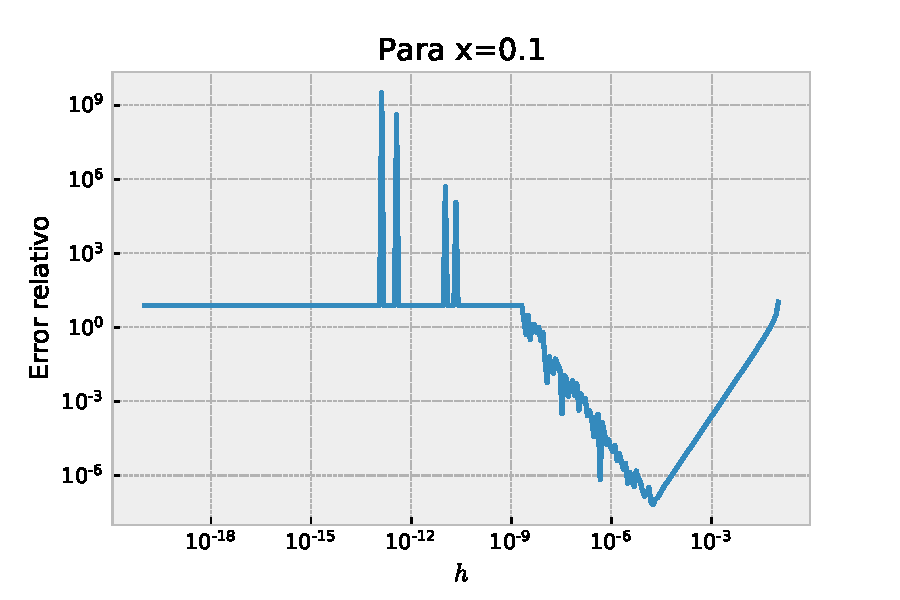
\includegraphics[width=\textwidth]{tex/img/graf0_1_deriv.pdf}
        \caption{}
        \label{graf1d}
    \end{subfigure}
    \hfill
    \begin{subfigure}[b]{0.3\textwidth}
        \centering
        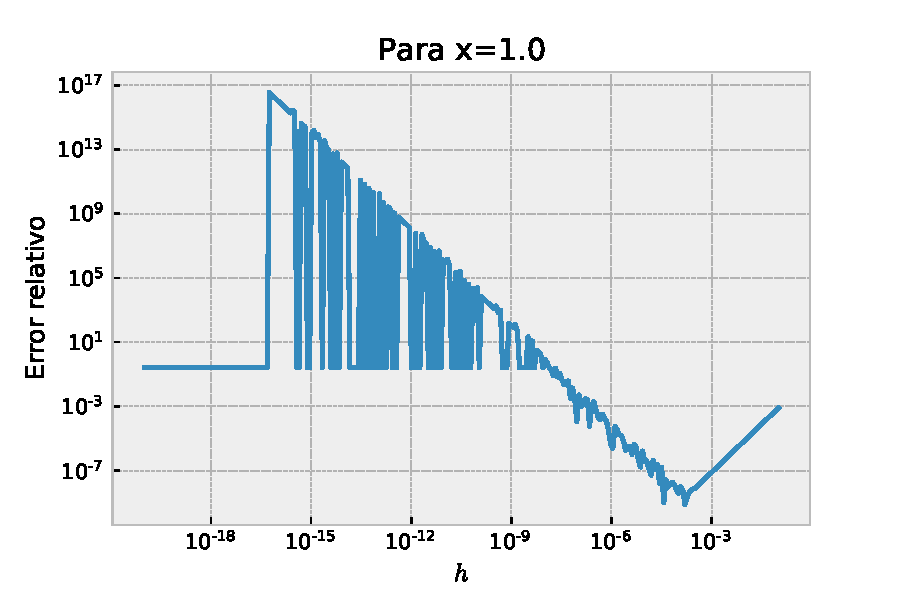
\includegraphics[width=\textwidth]{tex/img/graf1_0_deriv.pdf}
        \caption{}
        \label{graf2d}
    \end{subfigure}
    \hfill
    \begin{subfigure}[b]{0.3\textwidth}
         \centering
         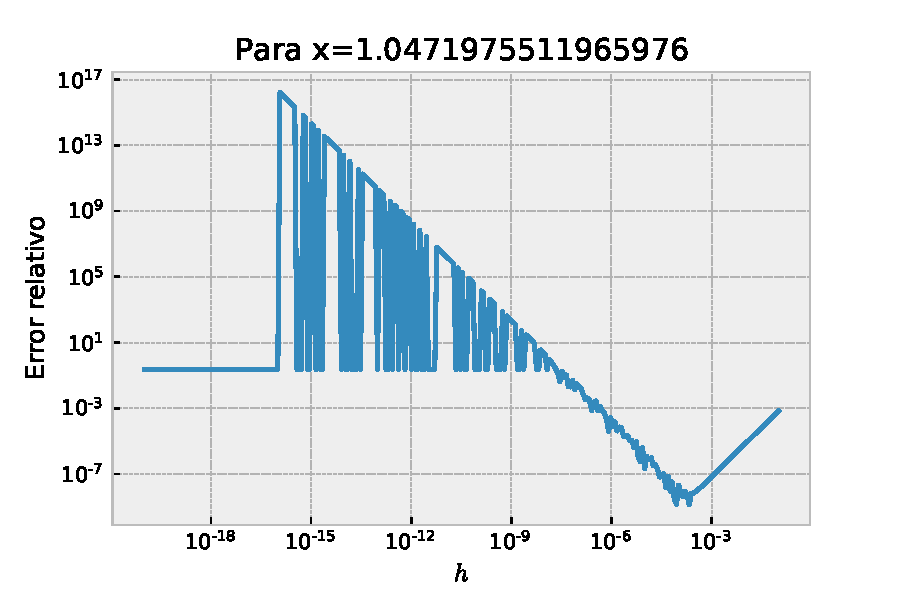
\includegraphics[width=\textwidth]{tex/img/graf1_0471975511965976_deriv.pdf}
         \caption{}
         \label{graf3d}
     \end{subfigure}
    \caption{Gráficos de error relativo v/s $h$ para los distintos valores de $x=\{ 0$.$1 , 1, \pi/3   \}$.}
    \label{graf123d}
\end{figure}

\subsection{Conclusión}
En este laboratorio se demostró que la segunda derivada centrada de una función puede ser escrita como \ref{deriv2cent}, luego se estudio el error en función de $h$ de la segunda derivada numérica y analítica de la función $f(x)= \sqrt{x}$, obteniéndose el valor más óptimo para $h$ para distintos valores de $x$. 

\vspace{2mm}
Antes de realizar este laboratorio pensaba que mientras más pequeño era el valor de $h$ que se le entregaba al computador más exacto iba a ser el resultado que se iba a obtener, pero esto no es así, pues el computador no trabaja bien con números extremadamente pequeños.
Por otra parte, aprendí sobre las derivadas adelantadas y retrasadas y que se pueden aplicar en métodos numéricos para programar.

\vspace{2mm}
Creo que faltó trabajar un poco en los errores y cómo estos se calculan, ya que no me quedaron muy claros. También creo que entender este laboratorio en clases se me hizo más complicado de lo que debería ya que recordaba muy poco de python y específicamente de cómo utilizar \texttt{matplotlib}, pues si mal no recuerdo en el ramo de computación científica no se alcanzó a ver bien este paquete.
\end{document}
